\chapter{Implémentation naïve et optimisations}

\section{Méthode de calcul brute}
La méthode de résolution dite naïve ou brute est la méthode de calcul la plus intuitive mais aussi la plus inefficace. Elle consiste simplement à calculer pour chaque particule les forces qui sont appliquées par toutes les autres. La complexité d'un tel calcul est en $O(N^2)$, il paraît alors évident que cette méthode de calcul est vraiment inefficace.

Voici par exemple, le résultat que nous obtenons avec cette méthode :

\begin{center}
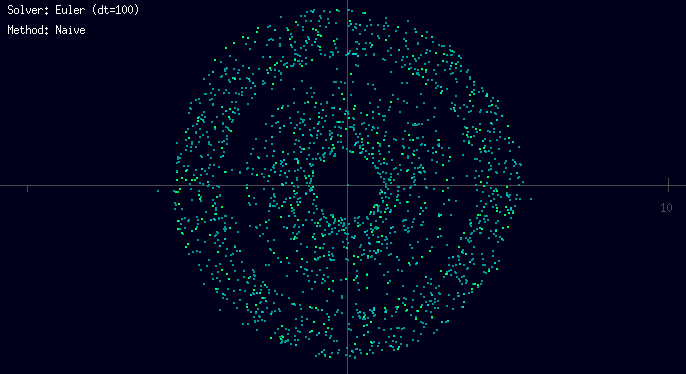
\includegraphics[scale=0.8]{images/naive.png}
\captionsetup{hypcap=false}
\captionof{figure}{Méthode naïve avec 1000 particules}
\label{fig2}
\end{center}

On observe ainsi, que les interactions entre particules semblent cohérentes ce qui laisse apparaître une petite galaxie.

En terme de performance, comme prévu l'algorithme est inefficace et montre ses limites pour $N>1000$ ce qui est bien trop petit pour pouvoir simuler des galaxies.

\section{Optimisation de la méthode de calcul brute}
\vspace{2mm}
Une première manière d'optimiser le calcul des forces est d'utiliser le principe d'action-réaction afin de ne pas effectuer plusieurs fois les calculs.
Pour cela, nous pouvons suivre une démarche d'optimisation dynamique en utilisant plus de mémoire afin de réduire nos calculs. Ainsi, en stockant nos forces successives dans un tableau, nous pouvons éviter de faire des calculs déjà effectués.

\vspace{2mm}
Cela donne donc le nombre de calculs suivant :
\vspace{1mm}

$C=\sum_{n=1}^N n = \frac{N(N-1)}{2}$

\vspace{2mm}
On peut déjà observer que la complexité de ce calcul est toujours  en $O(N^2)$ mais qu'utiliser cette méthode permet de diviser le nombre de calculs par $2$ ce qui est déjà une optimisation intéressante. Cependant, étant donné que l'on garde toujours une complexité quadratique, cela n'est toujours pas suffisamment efficace pour simuler des galaxies. En pratique, nous pouvons simuler $2000$ particules tout en ayant de bonnes performances mais au-delà de $2000$, la méthode montre ses limites.

\begin{center}
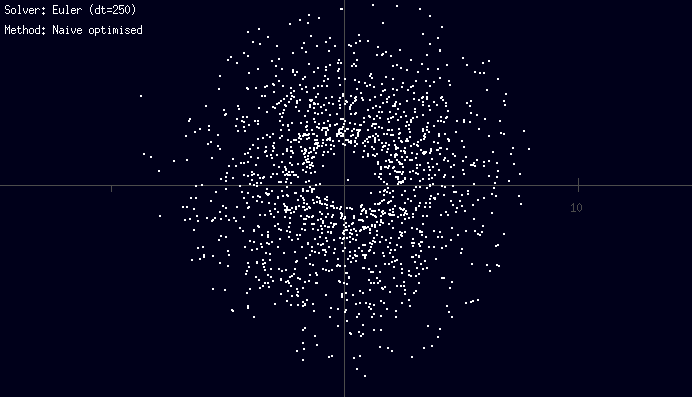
\includegraphics[scale=0.8]{images/naive_optimised.png}
\captionsetup{hypcap=false}
\captionof{figure}{Méthode naïve optimisée avec 2000 particules}
\label{fig3}
\end{center} 

\begin{center}
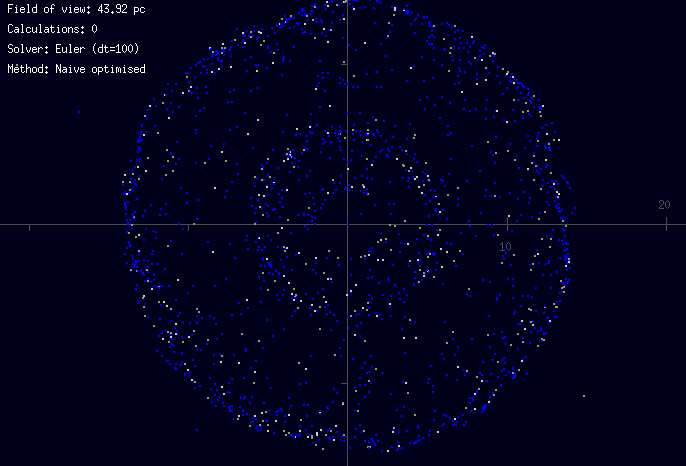
\includegraphics[scale=0.8]{images/NO.png}
\captionsetup{hypcap=false}
\captionof{figure}{Méthode naïve optimisée avec 2000 particules colorées}
\label{fig4}
\end{center} 


